% jgb: Proposal for the text above
In this section we show the results of our study, answering the research questions presented in the introduction. 
The following results are intended to determine the extent to which we can operationalize the theoretical model proposed by \gema~
We have considered a total of 809 bugs in the Defects4J dataset, after filtering out bugs for the four projects we do not consider as explained in Section~\ref{subsec:dataset}. The results we found for each of those bugs are summarized in Figure~\ref{fig:experiment-overview}. 
This figure differentiates the cases in which, out of the total number of bugs, the regression test was found to pass again in some commit prior to the BFC from those that did not. In turn, from this first group, we differentiate the bugs from which we have been able to obtain a single candidate to be the BIC or several of them.
%\as{I guess that this figure should be somehow discussed?}
%\michel{I add a little explanation}

\begin{figure}[h!]
    \centering    
    % \begin{tikzpicture}[node distance=1cm,every node/.style={fill=white, font=\sffamily}, align=center]
%     % Specification of nodes (position, etc.)
%     \node (total)             [large]                                         { };
%     \node (buildable)         [large, below of=total]                         { };
%     \node (testBuildable)     [large, below of=buildable]                     { };
%     \node (success)           [large, below of=testBuildable]                 { };

%     \draw[-Latex]             (total) -- (buildable);
%     \draw[-Latex]             (buildable) -- (testBuildable);
%     \draw[-Latex]             (testBuildable) -- (success);

% \end{tikzpicture}
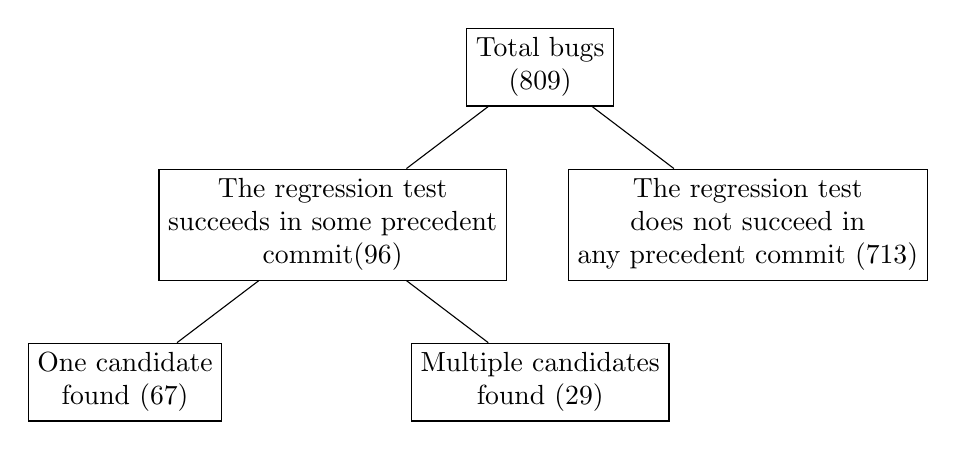
\begin{tikzpicture}[sibling distance=15em, level distance=2cm,
    every node/.style = {shape=rectangle, draw, align=center, top color=white,  }]
    \node {Total bugs \\ (809)}
      child { node {The regression test \\ succeeds in some precedent\\ commit(96)} 
          child { node {One candidate\\ found (67)} }
          child { node {Multiple candidates\\ found (29)} }
      }
      child { node {The regression test\\ does not succeed in\\  any precedent commit (713)} }
      ;
\end{tikzpicture}
  %  \vspace{-0.5cm}
    \caption{Summary of results for each of the bugs considered in the study.}
    \label{fig:experiment-overview}
\end{figure}

%%%%%%%%%%%%%
%    RQ1A    %
%%%%%%%%%%%%%

\subsection{\rqonea}
\label{results:rq1a}

In Table~\ref{table:results-per-project} we show the values for each of the interpretations of Transplantability for each bug. 
The values are aggregated by project, showing the mean and median for all bugs in each project. 
%The table also provides the aggregation of all bugs from all projects to obtain the mean and median Transplantability values for the dataset.
Additionally, we add in the table the relative position (\%) of commit $n$ (1) with respect to the total number of days elapsed between the BFC and the first commit of the project and (2) with respect to the total number of commits between the BFC and the first commit of the project. 
A value close to 0\% in this relative position indicates that we have barely been able to transplant the regression test, while values close to 100\% indicate that the test has been transplanted in most of the past (with respect to the BFC).

\begin{table*}[ht!]
    \caption{\label{table:rq1a} Transplantability (in days and in number of commits) for each bug, aggregated by mean ({\large $\mean{x}$}), 
    by median ({\large $\median{x}$}) and by the relative position of the oldest commit where the test could be transplanted ({$\%$}).}
    \resizebox{\textwidth}{!}{%
        \begin{tabular}{|r|r|rrr|rrr|}
            \hline
            \multicolumn{1}{|c|}{}                 &                  & \multicolumn{3}{c|}{$T_{days}$}                                                   & \multicolumn{3}{c|}{$T_{commmits}$}\\
            %\cline{3-8} \\
            \multicolumn{1}{|c|}{\textbf{Project}} & \textbf{\# bugs} & \multicolumn{1}{c|}{\textbf{\large{\large $\mean{x}$}}} & \multicolumn{1}{c|}{\textbf{\large{\large $\median{x}$}}} & \multicolumn{1}{c|}{\textbf{\%}} & \multicolumn{1}{c|}{\textbf{\large{\large $\mean{x}$}}} & \multicolumn{1}{c|}{\textbf{\large{\large $\median{x}$}}} & \multicolumn{1}{c|}{\textbf{\%}} \\ \hline
            \textbf{Cli}                            & 39                                     & \multicolumn{1}{r|}{910}  & \multicolumn{1}{r|}{1168} & 36.09                 & \multicolumn{1}{r|}{134}  & \multicolumn{1}{r|}{115}  & 34.67                 \\ \hline
            \textbf{Closure}                        & 174                                    & \multicolumn{1}{r|}{234}  & \multicolumn{1}{r|}{108}  & 36.63                 & \multicolumn{1}{r|}{451}  & \multicolumn{1}{r|}{187}  & 39.62                 \\ \hline
            \textbf{Codec}                          & 18                                     & \multicolumn{1}{r|}{703}  & \multicolumn{1}{r|}{427}  & 27.06                 & \multicolumn{1}{r|}{192}  & \multicolumn{1}{r|}{78}   & 26.12                 \\ \hline
            \textbf{Collections}                    & 4                                      & \multicolumn{1}{r|}{599}  & \multicolumn{1}{r|}{703}  & 11.05                 & \multicolumn{1}{r|}{178}  & \multicolumn{1}{r|}{213}  & 6.30                  \\ \hline
            \textbf{Compress}                       & 47                                     & \multicolumn{1}{r|}{1885} & \multicolumn{1}{r|}{2021} & 47.64                 & \multicolumn{1}{r|}{1223} & \multicolumn{1}{r|}{1326} & 82.18                 \\ \hline
            \textbf{Csv}                            & 16                                     & \multicolumn{1}{r|}{106}  & \multicolumn{1}{r|}{41}   & 3.11                  & \multicolumn{1}{r|}{41}   & \multicolumn{1}{r|}{27}   & 5.17                  \\ \hline
            \textbf{Gson}                           & 18                                     & \multicolumn{1}{r|}{1283} & \multicolumn{1}{r|}{1212} & 47.60                 & \multicolumn{1}{r|}{481}  & \multicolumn{1}{r|}{368}  & 41.70                 \\ \hline
            \textbf{JacksonCore}                    & 26                                     & \multicolumn{1}{r|}{444}  & \multicolumn{1}{r|}{450}  & 32.98                 & \multicolumn{1}{r|}{262}  & \multicolumn{1}{r|}{258}  & 34.00                 \\ \hline
            \textbf{JacksonDatabind}                & 112                                    & \multicolumn{1}{r|}{718}  & \multicolumn{1}{r|}{666}  & 43.92                 & \multicolumn{1}{r|}{1183} & \multicolumn{1}{r|}{1123} & 40.74                 \\ \hline
            \textbf{JacksonXml}                     & 6                                      & \multicolumn{1}{r|}{884}  & \multicolumn{1}{r|}{939}  & 40.49                 & \multicolumn{1}{r|}{256}  & \multicolumn{1}{r|}{239}  & 40.41                 \\ \hline
            \textbf{Jsoup}                          & 93                                     & \multicolumn{1}{r|}{437}  & \multicolumn{1}{r|}{240}  & 26.95                 & \multicolumn{1}{r|}{142}  & \multicolumn{1}{r|}{76}   & 18.33                 \\ \hline
            \textbf{JxPath}                         & 22                                     & \multicolumn{1}{r|}{607}  & \multicolumn{1}{r|}{532}  & 24.44                 & \multicolumn{1}{r|}{80}   & \multicolumn{1}{r|}{79}   & 21.65                 \\ \hline
            \textbf{Lang}                           & 64                                     & \multicolumn{1}{r|}{355}  & \multicolumn{1}{r|}{246}  & 14.88                 & \multicolumn{1}{r|}{283}  & \multicolumn{1}{r|}{206}  & 13.05                 \\ \hline
            \textbf{Math}                           & 106                                    & \multicolumn{1}{r|}{186}  & \multicolumn{1}{r|}{110}  & 7.60                  & \multicolumn{1}{r|}{280}  & \multicolumn{1}{r|}{178}  & 10.16                 \\ \hline
            \textbf{Mockito}                        & 38                                     & \multicolumn{1}{r|}{1664} & \multicolumn{1}{r|}{1552} & 96.61                 & \multicolumn{1}{r|}{1781} & \multicolumn{1}{r|}{1540} & 95.93                 \\ \hline
            \textbf{Time}                           & 26                                     & \multicolumn{1}{r|}{452}  & \multicolumn{1}{r|}{478}  & 28.02                 & \multicolumn{1}{r|}{97}   & \multicolumn{1}{r|}{77}   & 19.33                 \\ \hline
            \hline
            \textbf{All bugs}                       & 809                                    & \multicolumn{1}{r|}{585}  & \multicolumn{1}{r|}{302}  & 32.93                 & \multicolumn{1}{r|}{530}  & \multicolumn{1}{r|}{212}  & 33.83                 \\ \hline
        \end{tabular}
    }
\end{table*}


For a more comprehensive view of the Transplantability results, Table~\ref{table:rq1a-iqr} provides in detail the distribution of $T_{days}$ and $T_{commits}$ results.
First, we found that both metrics offer very similar results, showing that the average frequency with which a commit is added to these repositories is approximately 1 day. 
% \michel{Here I think a reviewer could tell us why we use two metrics that mean the same thing. Although it may seem intuitive, I have read other articles about the frequency of commits per day in open source projects and they are around 4 commits/day on average.}\as{I think that this was some of Gregorio's work? We need to comment on this.}
Regarding the minimum value for both metrics, we found the value 0, which indicates that for at least one project, it was not possible to transplant the test to the commit prior to the BFC. We found that for bug 79 of the Closure project the BFC includes a new function as part of the bug fix, being this function used in the regression test. Since this function does not exist in the previous commits to the BFC, the error obtained when transplanting the test to them is a failure in the compilation of the test code.

\begin{table*}[]
    \caption{\label{table:rq1a-iqr} Distribution of Transplantability results for all projects}
    \resizebox{\textwidth}{!} & \textbf{50\%} & \textbf{75\%} & \textbf{max} \\ \hline
      \textbf{$T_{days}$}    & 809              & 585           & 706          & 0            & 84            & 302           & 830           & 3,475         \\ \hline
      \textbf{$T_{commits}$} & 809              & 530           & 696          & 0            & 72            & 212           & 712           & 3,709         \\ \hline
      \end{tabular}
    }
\end{table*}

In order to evaluate the feasibility of our method, we check whether the BIC found by our tool falls within the $T_{commits}$ and $T_{days}$ for the different regression tests. In this case we can assume that, at least for the considered projects, the test can be transplanted far enough to allow the detection of the BIC. 
For the 67 BICs detected, we found that, on mean, they are 182 days  and 190 commits between the BIC and the BFC. 
The diversity of projects forces us to check, in addition, the median: 47 days and 49 commits respectively. 
According to the values of $T_{days}$ and $T_{commits}$ we can state that we have been able to transplant the regression tests far enough to be useful in detecting the BIC. 
%\as{This is an extremely bold statement. To claim usefulness we need to somehow hear this from the developers of the original projects but this is probably impossible since the data is likely to be old. Is there a way to say something about ``far enough'' without asking developers?}
%\michel{We rephrased the statement to focus on the ``feasibility'' of the method}

Nevertheless, there might be commits between $n$ and the BFC where the regression test cannot be compiled or run. This leads us to the next RQ.

\vspace{0.4cm}
\fbox{\begin{minipage}{0.9\textwidth}
    \textbf{\rqonea}
    For the dataset used, we have managed to transplant the regression test for a bug up to 585 days (530 commits) in the past on average. 
    For 50\% of the bugs, the regression test could be transplanted up to at least 302 days (212 commits).
    On average, regression tests can be transplanted to a 32.93\% of the days (33.83\% of the commits) between the BFC and the initial commit of the project.
\end{minipage}}

%%%%%%%%%%%%%
%    RQ1B    %
%%%%%%%%%%%%%

\subsection{\rqoneb}
\label{results:rq1b}

In Table~\ref{table:results-per-project} we show average and mean data for the three metrics defined in Section~\ref{sec:bug-hunter:methodology}: source compilability, transplanted test compilability and transplanted test runnability.

\begin{table}[h!]
    \centering{\small
        \caption{\label{table:results-per-project} Source code compilability, transplanted test compilability, and transplanted test runnability for each bug, aggregated by mean ({\large $\mean{x}$}) and by median ({\large $\median{x}$}) per project. 
        Values are shown in percentages.}
        \begin{tabular}{|r|r|rr|rr|rr|}
            \hline
            \multicolumn{1}{|c|}{\multirow{2}{*}{\textbf{Project}}} & \multicolumn{1}{c|}{\multirow{2}{*}{\textbf{\# bugs}}} & \multicolumn{2}{c|}{\textbf{\begin{tabular}[c]{@{}c@{}}Source \\ Compilability\end{tabular}}} & \multicolumn{2}{c|}{\textbf{\begin{tabular}[c]{@{}c@{}}T.Test \\ Compilability\end{tabular}}} & \multicolumn{2}{c|}{\textbf{\begin{tabular}[c]{@{}c@{}}T.Test \\ Runnability\end{tabular}}} \\ %\cline{3-8} 
            \multicolumn{1}{|c|}{}                                  & \multicolumn{1}{c|}{}                                     & \multicolumn{1}{c|}{\textbf{\large{\large $\mean{x}$}}}     & \multicolumn{1}{c|}{\textbf{{\large $\median{x}$}}}    & \multicolumn{1}{c|}{\textbf{{\large $\mean{x}$}}}    & \multicolumn{1}{c|}{\textbf{{\large $\median{x}$}}}   & \multicolumn{1}{c|}{\textbf{{\large $\mean{x}$}}}   & \multicolumn{1}{c|}{\textbf{{\large $\median{x}$}}}   \\ \hline
            \textbf{Cli}                            & 39                                     & \multicolumn{1}{r|}{56.07} & 62.61                 & \multicolumn{1}{r|}{29.40} & 30.88                 & \multicolumn{1}{r|}{29.40} & 30.88                 \\ \hline
            \textbf{Closure}                        & 174                                    & \multicolumn{1}{r|}{59.24} & 54.36                 & \multicolumn{1}{r|}{33.52} & 17.63                 & \multicolumn{1}{r|}{33.52} & 17.63                 \\ \hline
            \textbf{Codec}                          & 18                                     & \multicolumn{1}{r|}{28.30} & 14.29                 & \multicolumn{1}{r|}{25.13} & 8.84                  & \multicolumn{1}{r|}{25.13} & 8.84                  \\ \hline
            \textbf{Collections}                    & 4                                      & \multicolumn{1}{r|}{97.94} & 98.98                 & \multicolumn{1}{r|}{5.73}  & 7.46                  & \multicolumn{1}{r|}{5.61}  & 7.37                  \\ \hline
            \textbf{Compress}                       & 47                                     & \multicolumn{1}{r|}{29.96} & 23.60                 & \multicolumn{1}{r|}{20.81} & 17.02                 & \multicolumn{1}{r|}{18.35} & 10.22                 \\ \hline
            \textbf{Csv}                            & 16                                     & \multicolumn{1}{r|}{19.07} & 17.38                 & \multicolumn{1}{r|}{5.26}  & 3.51                  & \multicolumn{1}{r|}{5.21}  & 3.51                  \\ \hline
            \textbf{Gson}                           & 18                                     & \multicolumn{1}{r|}{42.00} & 35.98                 & \multicolumn{1}{r|}{40.73} & 34.68                 & \multicolumn{1}{r|}{40.73} & 34.68                 \\ \hline
            \textbf{JacksonCore}                    & 26                                     & \multicolumn{1}{r|}{35.08} & 32.54                 & \multicolumn{1}{r|}{31.52} & 30.12                 & \multicolumn{1}{r|}{31.52} & 30.12                 \\ \hline
            \textbf{JacksonDatabind}                & 112                                    & \multicolumn{1}{r|}{88.37} & 90.17                 & \multicolumn{1}{r|}{13.77} & 14.22                 & \multicolumn{1}{r|}{13.77} & 14.22                 \\ \hline
            \textbf{JacksonXml}                     & 6                                      & \multicolumn{1}{r|}{89.65} & 88.81                 & \multicolumn{1}{r|}{24.49} & 24.59                 & \multicolumn{1}{r|}{24.49} & 24.59                 \\ \hline
            \textbf{Jsoup}                          & 93                                     & \multicolumn{1}{r|}{21.08} & 12.52                 & \multicolumn{1}{r|}{17.56} & 9.74                  & \multicolumn{1}{r|}{17.56} & 9.74                  \\ \hline
            \textbf{JxPath}                         & 22                                     & \multicolumn{1}{r|}{92.25} & 100.00                & \multicolumn{1}{r|}{21.93} & 23.57                 & \multicolumn{1}{r|}{21.93} & 23.57                 \\ \hline
            \textbf{Lang}                           & 64                                     & \multicolumn{1}{r|}{74.08} & 66.08                 & \multicolumn{1}{r|}{11.61} & 8.50                  & \multicolumn{1}{r|}{11.61} & 8.50                  \\ \hline
            \textbf{Math}                           & 106                                    & \multicolumn{1}{r|}{39.80} & 36.19                 & \multicolumn{1}{r|}{7.99}  & 5.86                  & \multicolumn{1}{r|}{7.99}  & 5.86                  \\ \hline
            \textbf{Mockito}                        & 38                                     & \multicolumn{1}{r|}{30.69} & 30.06                 & \multicolumn{1}{r|}{24.17} & 25.22                 & \multicolumn{1}{r|}{24.17} & 25.22                 \\ \hline
            \textbf{Time}                           & 26                                     & \multicolumn{1}{r|}{72.84} & 100.00                & \multicolumn{1}{r|}{20.72} & 6.47                  & \multicolumn{1}{r|}{18.89} & 4.12                  \\ \hline
            \hline
            \textbf{All}                            & 809                                    & \multicolumn{1}{r|}{53.43} & 49.89                 & \multicolumn{1}{r|}{20.92} & 12.36                 & \multicolumn{1}{r|}{20.71} & 12.00                 \\ \hline
        \end{tabular}
    }
    \vspace{-4mm}
\end{table}


Table~\ref{table:rq1b-iqr} provides in detail the distribution these metrics for a more comprehensive view of the results. 

\begin{table}[]
  \caption{\label{table:rq1b-iqr} Distribution of source compilability, transplanted test compilability and transplanted test runnability results for all projects}
  \resizebox{\textwidth}{!} & \textbf{50\%} & \textbf{75\%} & \textbf{max} \\ \hline
      \textbf{Src compilability}      & 809              & 53.43         & 32.26        & 0.26         & 24.88         & 49.89         & 84.45         & 100.0        \\ \hline
      \textbf{T.Test compilability}   & 809              & 20.92         & 23.93        & 0.10         & 4.26          & 12.36         & 26.67         & 100.0        \\ \hline
      \textbf{T.Test runnability}     & 809              & 20.71         & 23.98        & 0.10         & 4.12          & 12.00         & 26.58         & 100.0        \\ \hline
    \end{tabular}
  }
\end{table}

The reasons that prevent transplanting the regression test are directly related to these metrics and can be classified as follows:

\begin{itemize}
\item \textbf{Compilability of the source code} If the source code cannot be built for the snapshot, there is no way to build the regression test. 
Compilability of past snapshots has been studied in detail by Tufano et al.~\cite{tufano2017there},whose experiment in 2014 showed an average compilability of 100 Java projects of 37.74\%. Maes-Bermejo et al.~\cite{maes2022revisiting} replicated this experiment in 2020 and a decrease in compilability was observed due to the lapse of time, 
%\as{Please be more explicit why the lapse of time could be expected to reduce the compilability value.} \michel{Below it is commented that one of the factors affecting compilability is the passage of time. I clarify it} 
obtaining a value of 25.09\%. The compilability may vary largely from project to project, and it will depend among other factors on the availability of third party modules needed to build the code, on the availability of the building tools in the right version, and on the complete automation of the building process. These factors are usually affected by time, and a degradation of compilability as time passes has been observed in these two previous studies
In our case, the mean compilability of the snapshots previous of each bug is 53.43\% (with a median of 49.89\%). 
The value obtained is higher than that obtained in previous studies due to a combination of good practices by the authors of the Defects4J dataset; 
% \as{do you mean that storing dependencies and adding configuration files are the good practices? Or are there some good practices (whatever they might be) and on top of them the developers store dependencies and adapt configuration files?}
% \michel{The configuration files and the storage of the libraries are the best practices that I want to emphasize. Further on I comment that it provides a high reproducibility of the experiments (understanding that these are good practices to follow for anyone who wants to make his dataset reproducible).} 
storing project dependencies and adapting their configuration files to ensure high reproducibility in the experiments (although only in the BFCs), together with additional adaptations made by the authors of this work, completing the adaptation of the configuration of each project to each commit of its history.
%\as{"relatively low" suggests comparison with some kind of baseline. How do our figures compare to those reported in the previous papers [36,22]?}
%\michel{Now is more clear and we have added the comparison with the previous studies + the reason why our results are higher + explain the modifications to improve the compilability.}
\item \textbf{Compilability of the regression test} If the test cannot be built, it cannot be run. The test is built on top of the snapshot, and it may not build because the code it expects in the snapshot is not present. This may happen because that code was still not implemented for a given snapshot. For example, this is the case if the test tests a certain function: in some past snapshot the function may not be implemented yet. This may also happen because the code was in the snapshot, but not in the way the test expects it. For example, this may happen in case of refactoring between the snapshot we are trying to build and the snapshot for which the test was designed. In general, these problems will be increasingly frequent for older commits with respect to the BFC, since more artifacts (code files, libraries or configuration files) could change since those snapshots to the one corresponding to the BFC, for which the regression test was designed. They will also be frequent in branches which for some reason lack some code needed by the test.
The aggregate results for the transplanted test compilability (20.92\% mean and 12.36\% median for all bugs) are strictly lower than source code compilability, since compiling the source code is a necessary step to be able to compile and run the tests. 
To the best of our knowledge, there is no large-scale study on the compilability of a test that is transplanted to past commits, so we do not have a baseline on which to compare the results obtained on this metric.
% \as{Can we find some kind of baseline to compare these numbers, similarly to the compilability figures for the source code?}
% \michel{There are no previous studies that transplant tests into the past and measure how far they can be taken. The closest is a study of ours (not yet published) in which we ran tests on all commits of a project.}
% \as{Can we comment that there is no publicly available baseline?}

\item \textbf{Runnability of the regression test} Even if the regression test can be built, maybe its run does not produce a result, but fails earlier due to some code not behaving as expected. 
% This may happen, for example, if the test calls some function that is expected to return a certain value, but returns some other because that was the case in the earlier version of the code corresponding to the snapshot. 
When aggregating all bugs together, the mean for transplanted test runnability is 20.71\%, and the median is 12\%. 
Which means that in half of the bugs the test could be transplanted successfully to less than 12\% of the commits (although the difference with the mean shows how in some bugs, the transplant was successful in a much higher fraction of the cases). 
These values are again slightly lower than the previous metric (the compilability of the regression test) since we need to compile the test code in order to be able to run it. In this case, the values are very close (or even equal) to those of the compilability of the regression tests, so we can affirm that if the transplanted test is successfully compiled, it can be executed.
Again, as far as we know, the runnability of a test transplanted to the past has not been addressed on a large scale.
Again, to the best of our knowledge, the runability of a test transplanted to the past has not been previously addressed.
% \as{Also here, no other baselines?}
% \michel{Like the previous one, we have no previous study to compare ourselves with.}
% \as{As above?}
% In some projects, transplanting bugs to past commits usually works, with medians as high as 98.07\% in Gson, meaning that in this case for half the bugs tests could be transplanted to almost all commits. But in others, it rarely works, such as in Collections or Csv, where in half the bugs the test could be transplanted to less than 4\% of the commits.
\end{itemize}

We will discuss the problems of transplanting the tests in the past in more detail in Section~\ref{sec:transplant-discuss}.
% \michel{Initially, the (specific) problems why I could not transplant the test to the past belonged to the discussion. In this section we start from metrics (src/test compilability and runnability) and delve (not too much) into the reasons why they do not obtain higher values. In the specified section I describe in more detail which problems I found and how I solved them.}

When examining the numbers for each project, we can see how, even when it varies from project to project, transplanted test runnability is always very similar to transplanted test compilability, which means that if the test compiled, in general it runs. In other words: the main blocker for running a test is that the test does not compile. For compiling the test, we should compile the source code. Again, by looking at this table, we can see how in some cases, the blocker for compiling the transplanted test is that the snapshot does not compile (for example for Gson, in almost all commits for which the snapshot compiled, the test also compiled). But for most of them, even if the snapshot compiles, the test does not.

These results are relevant because they show that by improving the compilability of the source code, and of the regression test, we could improve transplanted test runnability, and therefore, the applicability of the perfect test method. They also show that some projects have a very low compilability. 
This may be due to age (See Table~\ref{table:dataset-table})
%\as{Maybe we need to describe each and every bug? In any case here we should refer to such a table/description...}
of those projects (maybe the developers of those projects were using old practices that do not interact well with modern tools), or to specific characteristics of those projects, that maybe could be fixed with more knowledge about their building configuration.

Despite all these factors, the fact that for some projects transplanted test runnability is high shows that at least in some cases the conditions to use the perfect test method with regression tests hold.

\vspace{0.4cm}
\fbox{\begin{minipage}{0.9\textwidth}
    \textbf{\rqoneb}
    The effectiveness of the transplant is limited by compilability issues unrelated to the transplanted test (the snapshot does not compile 
    46.57\% of the time) or by compilability of the transplanted test (the test does not compile 79.08\% of the time, essentially because of the limitation in compiling the source code or because it relies on missing code). However, we found that when the test compiles, in general, the test can be run. Therefore, compilability of the source code is a blocker that, when improved, could improve the transplanted test runnability.
\end{minipage}}

%%%%%%%%%%%%%
%    RQ2    %
%%%%%%%%%%%%%

\subsection{\rqtwo}
\label{sec:rq2}

Following on with the chart in Figure~\ref{fig:experiment-overview}, to answer $RQ_2$ we will study in which cases the test succeeded in some precedent commit, and in those cases, how many candidate BICs were found. We consider the following scenarios as defined in our methodology. 

\textbf{The test does not succeed in any previous commit.}

From the total 809 bugs, in 713 the regression test did not succeed in any commit previous to it. 
In these cases, the perfect test method (using regression test as perfect tests) does not allow us to identify candidates for being the BIC. 
Since the test never succeeds in commits previous to the BFC, we cannot find the commit in which the bug was introduced. 
In the snapshots corresponding to some of those commits this is because the test cannot be run (and therefore we don't know if the bug is present or not in them), and in some others because it can be run, but fails (and then we know that the bug is present).

The reasons for the test not running (the test was not successfully transplanted) were already explored in the previous section, and in many cases are related to compilability problems. 
The fact that the tests are executed (successfully transplanted) but fail in all commits prior to the BFC is a case contemplated and addressed by the perfect testing method: it means that the bug is present in those snapshots since the feature tested was introduced.
However, if we cannot find a previous commit for which the test succeeds, we have no evidence of where the BIC is.

\textbf{The test succeeds again in some past commit.}

For the remaining 96 bugs, the test succeeds in at least one commit previous to the BFC, and therefore we can provide more conclusive results by running the perfect test method.

For 67 bugs out of these 96, our algorithm produces a single candidate to be the BIC. 
The regression test succeeds in snapshots previous to this BIC candidate, which means it is the FFC (First-Failing Change), and following the perfect test method, the commit that introduce the bug (BIC). 
In 8 of these cases, the BIC was found in a direct parent of the BFC, which means the bug was detected and fixed very quickly after it was introduced. 
This is due to a practice known as \textit{Backtracking}~\cite{yoon2012exploratory,yoon2014longitudinal}, where the developer reverts part or all of the change made when an issue is reported.

For the 29 remaining bugs, the algorithm finds multiple candidates. 
If $n$ is the first commit (going backwards from the BFC) in which the test succeeds, we have several candidates if for one or more commits that are right before $n$ (again, going backwards from the BFC) the test could not be executed (we are not able to compile the code or the test).
In those cases, since the test could not be run, we do not know if the bug is present or not, and, according to the definition provided by~\gema, any of them could be the FFC (the first failing change).
So, all of them, including the last one that failed (again, in the same order), are possible BICs. 
Without more information, we cannot assess which one of them is really the BIC.

%\as{Is it possible that none of them is the BIC? If yes, ``which'' in the previous sentence might be a wrong word choice.}
%\michel{Given that there is a commit in the past where the test passes again (but in the commits following this one the test cannot be executed) and having verified that when the test can be executed, it locates the commit that introduced the error, we assume that indeed one of the candidates is the BIC. The Gem model does not contemplate that there is no BIC when we find a test that happens again in the past.}
%\as{Do we want to make this assumption explicit?}
%\michel{We rephrase stated that we follow the definition provided by Gema}

\vspace{0.4cm}
\fbox{\begin{minipage}{0.9\textwidth}
    \textbf{\rqtwo}
    Yes, at least for those cases where a functionality no longer behaves as the regression test expects it. 
    The regression test can be transplanted to past commits, and using the perfect test method with the regression test as perfect test, the BIC can be found. 
    In our case, for the 809 bugs for which we could assess the regression test detected the bug, we could use the method to identify precisely the BIC in 67 bugs, and to provide a list of candidates for other 29 bugs. 
    The bugs for which the method did not work were mainly due to not being able of running the test, because of compilability or runnability problems, in addition to the contemplated case in which the tested feature has always contained the bug
    In general, when regression tests could be run, the method worked.
\end{minipage}}

\subsection{Validation of results}

%\as{We seem to assume that BIC is (at least theoretically) unique but what if the bug is introduced through interplay between several commits?}
%\michel{As I understand Gema's model and how regression tests work, the first commit in which the test fails and its parent (or parents) have a success score on the same test should be the BIC. If there have been changes in different commits, our method will detect the first change that actually breaks the functionality as it is expected to work in the regression test.}
Once we have detected the BIC for 67 bugs through the perfect test method, we want to ensure that the BIC found is actually the BIC, the commit that introduced that bug. Following the steps already described in Section~\ref{sec:bug-hunter:methodology}, we checked manually all these cases, finding that all of them are true positives. This result allows for two conclusions:
\begin{itemize}
\item The perfect test method can be used to identify the bug introducing change, with regression tests as perfect tests, at least for those cases where a functionality no longer behaves as the regression test expects it.
\item We have a ground truth dataset of 67 bugs for which we know the BFC and the BIC, which can be used to evaluate methods for finding the BIC.
\end{itemize}

This manual analysis also allowed us to explore in some detail how those commits introduced the bug. We found the following two cases:
% \reviewer{This doesn't seem very insightful. One could consider that all commits are either bug fixes, refactorings or introducing new features. You find two out of three. Maybe it is surprising that you don't find new features that introduce bugs.  But the dataset is also pretty small.}
% \michel{If we consider a new feature such as, for example, adding additional cases within a function, then we have found it (See \url{https://github.com/FasterXML/jackson-databind/commit/a6443b2467542314065ce4545bfb52d5df2a76ed}). If the reviewer is referring to a new feature, such as a new module or class that would cause existing functionality to fail, we have found no cases.}

\begin{inparaenum}[\bf(1)]
\item \textbf{The bug is introduced in a commit marked as FIX}. 
This means that the commit was trying to fix another bug, but while doing that, it introduced a new one. For example, Bug 24 of the JacksonDatabind project has a BIC which is the BFC of another bug. 
The bug fixed in that BIC deals with date serialization, changing several classes for that. 
One of those commits, which is reverted in the BFC for Bug 24, was the one introducing that new bug.
Previous studies~\cite{guo2010characterizing,purushothaman2005toward,yin2011fixes} also state that bug-fixing commits are more likely to introduce a new bug in the software.
%\as{There is some research on fixes that introduce bugs, we need to cite it.}
%\michel{I have added some relevant citations. If you know of any more, do not hesitate to complete it.}

\item \textbf{The bug is introduced as a refactoring or reimplementation}. 
This case will be illustrated with Bug 23 of the Jsoup project (an HTML parser).
The bug is that the special entities that include numbers, to display fractions in HTML do not recognize the numbers, so they do not work as expected  (i.e., the string ``\&frac12'' should generate ``½'').
In the commit marked as BIC by our tool, there is a refactoring of the parse functionality, the main method of the library. 
This function goes from internally using the Parser class to using TreeBuilder (a new class). 
This refactoring brings with it the creation of new classes (that TreeBuilder needs to operate), among which we will highlight Tokeniser and CharacterReader.
In the BFC the method consumeLetterThenDigitSequence is added to the CharacterReader class, while in the Tokeniser class the call to consumeLetterSequence is changed by another one to the method consumeLetterThenDigitSequence (from CharacterReader) and solving the bug by considering numbers as part of an entity.

% For example, Bug 23 of the Jsoup project, has a BIC in which the commit message states that it is the refactoring of a functionality in which several classes are affected. 
% In the BFC for this bug, only one function is fixed, which is the one that makes the test pass again. 
% In fact, this bug was present in the code for 86 commits. 
% \as{Sorry, I do not understand what has happened here. Did the BIC perform refactoring incorrectly, inadvertently introducing a bug; or was BIC a correct refactoring and it preserved earlier behavior subsequently preserving an earlier bug as well?}
% \michel{The BIC is a refactoring of several classes. In one of them a regression was introduced by the developer}
% \as{Maybe state explicitly that a regression was introduced in one of the classes affected.}
\end{inparaenum}

%\jgb{This text below could be moved to the discussion, but I think that a least a short introduction should be here, because of the importance of this result.}

This manual validation shows one of the most important results of our study: a collection of bugs with an identification of the BIC that introduced them can be produced automatically from a collection of BFCs using the perfect test method, with regression tests as perfect tests. 
These collections could be used to produce ground truth datasets for evaluation analysis, as we do in this study, but also for any other study where a collection of BICs is needed, such as those on how bugs are introduced.
In this chapter we provide~\datasetName~as one of these collections obtained from the Defects4J bug dataset, with a total of 67 identified BICs.

%%% Local Variables:
%%% mode: latex
%%% TeX-master: "../../../Tesis.tex"
%%% End:
